\documentclass{article}
\usepackage[utf8]{inputenc}
\usepackage{amsmath}
\usepackage[tmargin=1in,bmargin=1in,lmargin=1.25in,rmargin=1.25in]{geometry}


\title{TMA4280 - Introduction to supercomputing \\
\large{Compulsory exercise 2}}
\author{Pål Christie Ryalen and Sindre Eskeland}
\date{\today}

\usepackage{natbib}
\usepackage{graphicx}

\setlength\parindent{0pt}

\begin{document}
\setcitestyle{square}
\maketitle



This is a compulsory exercise in the subject 'TMA4280 - Introduction to supercomputing' at NTNU. We will use the celebrated programming language C to calculate numerical solutions the Poisson problem

\begin{align}
    -\nabla^2 u & = f 	&\text{ in } \Omega = (0,1) \times (0,1)  \label{eqn:pois}\\ 
 u & = 0 			&\text{ on } \partial \Omega \label{eqn:bnd}
\end{align}

Where $f$ is a given function, while $u$ is sought. Our goal is to solve this problem using message passing interface(MPI) and the language extension OpenMP for parallel programming.  It is also of interest to compare computation time, as well as speedup and parallel efficiency with different number of MPI and OpenMP threads.


%%%%%%%%%%%%%%%%%%%%%%%%%%%%%%%%%%%%%%%%%%%%%%%%%%%%%%%%%%%%%%%%%%%
%%%%%%%%%%  discussion of possible solution strategies  %%%%%%%%%%%
%%%%%%%%%%%%%%%%%%%%%%%%%%%%%%%%%%%%%%%%%%%%%%%%%%%%%%%%%%%%%%%%%%%


\section{Discussion of possible solution strategies} \label{sec:strat}

It is well known that equation (\ref{eqn:pois}) and (\ref{eqn:bnd}) yields a linear system

\begin{align}
    \underline{A}\underline{U} = \underline{b} \label{eqn:donkaments}
\end{align}

where $\underline{A}$ was found by using the five-point formula, $\underline{b}$ is associated with $f$, and $\underline{U}$ is a the finite difference approximation of $u$. In our case, we pick an approximation grid which is equidistant in both directions. For the problem (\ref{eqn:pois}), the length parameter is $h = \frac{1}{n}$. The problem (\ref{eqn:donkaments}) is usually solved numerically by one of two solution methods; direct or iterative. We make a short discussion of the two methods in the following.
\
\\
\\
An iterative solution method finds the solution of (\ref{eqn:donkaments}) by splitting the matrix $\underline{A}$ into a sum of matrices and reorganising the problem. More specifically, $\underline{A}$ may be split into matrices $\underline{L} + \underline{D} + \underline{T}$, where $\underline{D}$ is diagonal, $\underline{L}$ is lower diagonal and $\underline{T}$ is upper diagonal. Here we have the common iteration schemes

\begin{align*}
    \underline{D} \underline{U}^{k+1} &= b - (\underline{L} + \underline{T})\underline{U}^k & \text{(Gauss-Jacobi)}.\\
    (\underline{L} + \underline{D})\underline{U}^{k+1} &= b - \underline{T}\underline{U}^k & \text{(Gauss-Seidel)}.
\end{align*}

While the Gauss-Jacobi method is rather strict - we are only guaranteed that it will work if $\underline{A}$ is strictly diagonally dominant - the Gauss-Seidel will only need $\underline{A}$ to be symmetric positive definite(SPD)\cite[p.~49]{solmeths}. It turns out that our problem will converge with the Gauss-Jacobi method even though our candidate $\underline{A}$ is not diagonally dominant, that being said, the convergence is slow. On the other hand, it is easy to parallelise. In contrast, the Gauss-Seidel method is hard to parallelise, since each iteration can immediately be reused. However, this problem can be alleviated if we are clever in the way we do the parallelisation.
\
\\
\\
On a positive remark, for iterative schemes we may choose storage method as we please. This will be useful when performing parallelisation. We may partition our problem in the following two ways; partitioning the matrix, or partitioning the domain $\Omega$. Using the commands
\begin{center}
    \verb MPI_Dims_create() \\
    \verb MPI_Cart_create()
\end{center}
we are able to organise the parallelisation. As none of the mentioned methods were chosen, we will not discuss this further. A candidate method is the famous Krylov methods, in particular the conjugate gradient(CG) method, which demands that the matrix $\underline{A}$ is SPD. We will not discuss this further.
\
\\
\\\
Of the direct methods, the method using the discrete sine transform is compelling. Owing to the fact that $\underline{A}$ is SPD, and that we are able to find a tensor product operator, we have an algorithm that scales well in both in terms of calculation and memory. We spell out how the method works in the following. Given a tensor product operator for $\underline{A}$, we may write system (\ref{eqn:donkaments}) on the equivalent form
\begin{align}
    \underline{V} \underline{X}  + \underline{X} \underline{V}^\top = \underline{B}, \label{eqn:vsomething}
\end{align}
where $\underline{V}$ is SPD. Since $\underline{V}$ has the eigen decomposition $\underline{V} = \underline{Q}^\top \underline{\Lambda} \underline{Q}$, where $\underline{Q}$ is orthogonal, and $\underline{\Lambda}$ is a diagonal matrix. We may rewrite equation (\ref{eqn:vsomething}) as
\begin{align}
    \underline{\Lambda} \underline{\tilde{X}} + \underline{\tilde{X}} \underline{\Lambda} = \underline{\tilde{B}}, \label{eqn:tildelambdax}
\end{align}
where $\underline{\tilde{B}} = \underline{Q}^\top \underline{B} \underline{Q}$. Calculating the product $\underline{Q}^\top \underline{B} \underline{Q}$ will usually demand a healthy $\mathcal{O}(N^3)$ operations. However, as luck would have it, we can use the discrete sine transform to improve the performance. Using the orthogonality of $\underline{Q}$ we have the relations
\begin{align*}
    \underline{Q} &= \sqrt{\frac{N}{2}}\underline{S}. \\
    \underline{Q}^\top &= \sqrt{\frac{2}{N}}\underline{S}^{-1}.
\end{align*}
The above relations will allow us the calculate
\begin{align*}
    \underline{\tilde{B}}^\top = \underline{S}^{-1}\Big( \big( \underline{S} \underline{B} \big) \Big)
\end{align*}
in an improved $\mathcal{O}(N^2 \log (N))$ operations. Similarly, owing to the fact that $\underline{\Lambda}$ is diagonal, we may solve the system (\ref{eqn:tildelambdax}) in $\mathcal{O}(N^2)$ operations, where the $i,j$-th component reads
\begin{align*}
    \tilde{x}_{i,j} = \frac{\tilde{b}_{i,j}}{\lambda_i + \lambda_j}.
\end{align*}
$\Lambda_i$ for $i=1,\cdots,N$ are the eigenvalues of $\underline{V}$. Lastly, remembering that $\underline{\tilde{X}} = \underline{Q}^\top \underline{X} \underline{Q}$, we solve the system
\begin{align*}
    \underline{X} = \underline{S}^{-1} \Big(\underline{S} \big(\underline{\tilde{X}}^\top \big) \Big)^\top
\end{align*}
in $\mathcal{O}(N^2 \log(N))$ operations. The solution method employed in this project is the discrete sine transform.

%%%%%%%%%%%%%%%%%%%%%%%%%%%%%%%%%%%%%%%%%%%%%%%%%%%%%%%%%%%%%%%%%%%
%%%%%%%%%%%%%%%%%%%%%%%%%%%%%%%%%%%%%%%%%%%%%%%%%%%%%%%%%%%%%%%%%%%


\section{A walkthrough of the \texttt{cmake}-file}

We state the relevant code lines in the \texttt{cmake}-file below, and give a short description after that.

\begin{enumerate}
    \item \label{enum:minreq} \texttt{cmake\_minimum\_required(VERSION 2.6)}
    \item \label{enum:lang} \texttt{enable\_language(C)}
    \item \label{enum:langF} \texttt{enable\_language(Fortran)}
    \item \label{enum:openmp} \texttt{option(ENABLE\_OPENMP "Enable OpenMP support?" ON)}
    \item \label{enum:mpi} \texttt{option(ENABLE\_MPI    "Enable MPI support?" ON)}
    \item \label{enum:mpiallow} \texttt{if(ENABLE\_MPI)}\\
         \text{ \hspace{1pt} } \texttt{find\_package(MPI)}\\
        \texttt{endif()}
    \item \label{enum:mpiallow2} \texttt{if(MPI\_FOUND)} \\
                                        \text{ \hspace{1pt} } \texttt{add\_definitions(-DHAVE\_MPI=1)} \\
                                        \text{ \hspace{1pt} } \texttt{set(INCLUDES \$\{INCLUDES\} \$\{MPI\_INCLUDE\_PATH\})} \\
                                        \text{ \hspace{1pt} } \texttt{set(DEPLIBS\_C \$\{DEPLIBS\_C\} \$\{MPI\_C\_LIBRARIES\})} \\
                                        \text{ \hspace{1pt} } \texttt{set(DEPLIBS\_F \$\{DEPLIBS\_F\} \$\{MPI\_Fortran\_LIBRARIES\})} \\
                                    \texttt{endif()}
    \item \label{enum:openmpallow}  \texttt{if(ENABLE\_OPENMP)} \\
                                        \text{ \hspace{1pt} } \texttt{find\_package(OpenMP)} \\
                                        \text{ \hspace{1pt} } \texttt{if(OPENMP\_FOUND)} \\
                                        \text{ \hspace{13pt} } \texttt{add\_definitions(-DHAVE\_OPENMP=1)} \\
                                        \text{ \hspace{13pt} } \texttt{set(CMAKE\_C\_FLAGS "\$\{CMAKE\_C\_FLAGS\} \$\{OpenMP\_C\_FLAGS\}")} \\
                                        \text{ \hspace{1pt} } \texttt{endif()} \\
                                        \texttt{endif()}
    \item \label{enum:include} \texttt{include\_directories(\$\{INCLUDES\})}
    \item \label{enum:addlib} \texttt{add\_library(common fst.f)} 
    \item \label{enum:exec} \texttt{add\_executable(poisson poisson.c)}
    \item \label{enum:execf} \texttt{add\_executable(poisson-f poisson.f)}
    \item \label{enum:link} \texttt{target\_link\_libraries(poisson common \$\{DEPLIBS\_C\})}
    \item \label{enum:linkf} \texttt{target\_link\_libraries(poisson-f common \$\{DEPLIBS\_F\})}
    \item \label{enum:prop} \texttt{set\_target\_properties(poisson PROPERTIES LINKER\_LANGUAGE C)}
\end{enumerate}
\
\\
In the line \ref{enum:minreq} we impose that the version is not too old. The command \ref{enum:lang} enables support for the language \texttt{C} in CMake. In \ref{enum:langF}, we have also included the support to the \texttt{Fortran}-language, since it is employed in the code for the discrete sine transform. In the lines \ref{enum:openmp} and \ref{enum:mpi} we allow support for OpenMP and MPI, respectively. In point \ref{enum:mpiallow} we load the MPI package if \texttt{ENABLE\_MPI} is \texttt{ON}. In the first place in point \ref{enum:mpiallow} we let the compiler know that we wish to compile with MPI. In the places below - the places that begin with \texttt{set(} - we tell the compiler where the MPI-libraries are found. The chunk \ref{enum:openmpallow} has the same purpose as \ref{enum:mpiallow} and \ref{enum:mpiallow2}, only this time for OpenMP. Point \ref{enum:include} sends the \texttt{INCLUDE} directories to the compiler. Point \ref{enum:addlib} adds the file \texttt{fst.f} into a library called \texttt{common}. The library will be linked to the executables, as will be decsribed soon. Point \ref{enum:exec} and \ref{enum:execf} adds executables for the \texttt{C}- and \texttt{Fortran}-code, respectively. The commands \ref{enum:link} and \ref{enum:linkf} links the \texttt{common}-library to the executables of the \texttt{C} and \texttt{Fortran} files, respectively. Lastly, the command in \ref{enum:prop} reassures that the \texttt{poisson}-executable is linked as a \texttt{C} program.


%%%%%%%%%%%%%%%%%%%%%%%%%%%%%%%%%%%%%%%%%%%%%%%%%%%%%%%%%%%%%%%%%%
%%%%%%%%%%%%%%%%%%%%%%%%%%%% Kong-lol %%%%%%%%%%%%%%%%%%%%%%%%%%%%
%%%%%%%%%%%%%%%%%%%%%%%%%%%%%%%%%%%%%%%%%%%%%%%%%%%%%%%%%%%%%%%%%%

\section{Regarding \texttt{kongull}}
As can be found in the webpage\cite{kongull}, \texttt{kongull} has the following key properties
\begin{enumerate}
    \item \label{enum:kongproc} 2 x AMD Opteron model 2431 6-core (Istanbul) processors.
    \item \label{enum:kongspeed} 2400 GHz core speed.
    \item \label{enum:kongfreq} 667 MHz (48 GiB nodes) or 800 MHz (24 GiB nodes) bus frequency.
\end{enumerate}
Property \ref{enum:kongproc} allows us to use $12$ processors per node, and maximum 4 nodes. To compile and execute we needed to run the following commands
\begin{align}
    &\texttt{module load intel/compilers/11.1.059}. \label{eqn:load} \\
    &\texttt{module load cmake}.\\
    &\texttt{CC=icc FC=ifort cmake . -DCMAKE\_BUILD\_TYPE=Release}.  \label{eqn:blah} \\
    &\texttt{make}                                                  \label{eqn:make} \\
    &\texttt{qsub job.sh}
\end{align}
To compile with \texttt{Fortran} on \texttt{kongull} it is important to use command (\ref{eqn:load}) to load a \texttt{Fortran} compiler, the number specifies a version with better performance just \texttt{module load intel}. Command (\ref{eqn:blah}) creates the \texttt{Makefile} which compiles with command (\ref{eqn:make}). To submit a job, a \texttt{shell}-script needs to be written. The \texttt{shell}-script contains information about number nodes, of MPI threads and OpenMP threads to be used. When using 1 MPI thread \texttt{kongull} can only use 1 node. So the maximum number of OpenMP threads with 1 MPI thread is $12$, this is because one can only specify the number of MPI threads per node on \texttt{kongull}. For more information about the \texttt{shell} script, see \cite{shell}.






%%%%%%%%%%%%%%%%%%%%%%%%%%%%%%%%%%%%%%%%%%%%%%%%%%%%%%%%%%%%%%%%%%
%%%%%%%%%%%%%% a short explanation of the finished program %%%%%%%
%%%%%%%%%%%%%%%%%%%%%%%%%%%%%%%%%%%%%%%%%%%%%%%%%%%%%%%%%%%%%%%%%%

\section{A short explanation of the finished program}
We created a program solving equation (\ref{eqn:pois}), with boundary conditions (\ref{eqn:bnd}) using the method described in section \ref{sec:strat}, and called it \texttt{poisson}.
The program itself is made by combining several functions, the most important ones are presented in table \ref{tab:explainfunc}. We were given functions for discrete sine transform, but this will not be discussed further.
\begin{table}[h]
%\centering
    \begin{tabular}{ll}
    \texttt{double solution(double x, double y)} & Takes coordinates, \texttt{x}, \texttt{y}, returns the  value \\ & of \texttt{u} at that coordinate. \\
    \texttt{double b\_func(double x,double y)} & Takes coordinates, \texttt{x}, \texttt{y}, returns the value of \\ &  \texttt{f} at that coordinate. \\
    \texttt{void domDivide(int size, int n, int **vec)} & Divides \texttt{n} points on the number of\\ &processors, \texttt{size}. Returns values  to the \\&  matrix \texttt{vec}. \texttt{vec[rank][0]},  \texttt{vec[rank][1]} \\ & gives the start- and end- point for processor \\ & \texttt{rank}. Size of \texttt{vec} should be \texttt{size}$\times$\texttt{2}.  \\
    \texttt{void paralleltransp(int size,int rank,}& Transposes the matrix \texttt{b}, with size \texttt{m}$\times$\texttt{l} globally.\\ \texttt{int m,int l,int **vec,double **b)} \\ 
    \texttt{void solvepoisson(int n,int size,int rank)} & Solves Poisson's equation, and compares the result\\& to the analytical solution.
    \end{tabular}
    \caption{Explanation of important functions in \texttt{poisson}.}
    \label{tab:explainfunc}
\end{table}
\texttt{poisson} takes no argument, and will calculate a numerical approximation of the solution, and compare it to the analytical solution for problem sizes $2^k, k \in \{2, \cdots ,14\}$. The problem sizes are not arbitrarily chosen, discrete sine transform needs to work on numbers of size $2^k-1$, thus $n-1$ is the number of internal nodes. To change which problem to solve, one can simply change the output of the \texttt{solution} and \texttt{b\_func} functions. \texttt{poisson} will abort if number of MPI-threads are larger than the problem size.
Figure \ref{fig:exrun} shows how \texttt{poisson} is used in the \texttt{terminal}, and what it returns.

\begin{figure}[h]
    \texttt{/dir\$ make \\
    /dir\$ OMP\_NUM\_THREADS=2 mpirun -np 3 poisson \\
    \begin{tabular}{lllll }
    numpts & numprs & numtrd & maxerr   &       time\\
    4   &    3  &     2 &      4.870972e-03  &  0.012758\\
    8   &    3  &     2 &      1.189740e-03  &  0.005394\\
    \vdots
    \end{tabular}
    }
    \caption{Example of how to run \texttt{poisson}, and what will be returned.}
    \label{fig:exrun}
\end{figure}
For an explanation of output-data, see table \ref{tab:explainout}.
\begin{table}[h]
    %\centering
    \begin{tabular}{ll}
    \texttt{numpts} & Number of interior points pluss one. \\
    \texttt{numprs} & Number of MPI-threads used.\\
    \texttt{numtrd} & Number of OpenMP-threads used.\\
    \texttt{maxerr} & Largest difference between numerical solution, and analytical solution.\\
    \texttt{time}   & Total computation time in second. \\
    \end{tabular}
    \caption{Explanation of output data from \texttt{poisson}.}
    \label{tab:explainout}
\end{table}
It is important to note that \texttt{poisson} is written to run with several MPI and OpenMP threads. A program written to use only MPI, OpenMP, or neither would outperform \texttt{poisson} when using the same number of threads. 

%%%%%%%%%%%%%%%%%%%%%%%%%%%%%%%%%%%%%%%%%%%%%%%%%%%%%%%%%%%%%%%%%%
%%%%%%%%%%%%%%%%%%%%%%% Numerical results %%%%%%%%%%%%%%%%%%%%%%%%
%%%%%%%%%%%%%%%%%%%%%%%%%%%%%%%%%%%%%%%%%%%%%%%%%%%%%%%%%%%%%%%%%%
\section{Numerical results}
All numerical results, both convergence and speedup analysis was found using \texttt{kongull}, with analytical solution $ u = x(1-x) \sin( \pi y) $, and $f = \sin(\pi y) (2+\pi^2x(1-x))$. The speedup, and parallel efficiency where also calculated. Speedup is defined as
\begin{align*}
S_p = \frac{t_1}{t_p}
\end{align*}
and parallel efficiency as
\begin{align*}
\eta_p = \frac{S_p}{p}
\end{align*}
where $t_p$ is run time with $p$ processors, $S_p$ is speedup with $p$ processors, and $\eta_p$ is parallel efficiency for $p$ processors. Speedup measures how much faster a program runs with $p$ processors, ideal speedup is when $S_p = p$. Parallel efficiency measures how well each processor is utilized. Perfect parallel efficiency is when $\eta_p = 1$. \\
\texttt{poisson} has a great weakness, it gets time results from one run through. The time results should be averaged over many runs. The results enclosed may therefore have considerable interference in run time.
%!!!!!!!!!!!!!!!!!!!!!!!!!!!Skrive om at programmet bare kjører en tid, og at det derfor kan være litt tilfeldighet inne i resultatene!!!!!!!!!!!!!!!
\subsection{Convergence analysis}
To show convergence, \texttt{poisson} was run with $p$ MPI-threads and $t$ OpenMP -threads, with $p\cdot t = 36$. The result is shown in figure \ref{fig:conv}.
\begin{figure}[h]
    \centering
    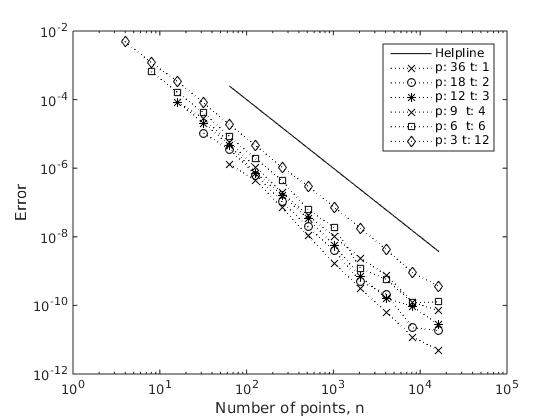
\includegraphics[width = 0.6\linewidth]{conv}
    \caption{A loglogplot of the convergence of \texttt{poisson}. The 'Helpline' shows the ideal convergence rate. The dotted lines shows the convergence rate for a certain number of MPI and OpenMP threads.}
    \label{fig:conv}
\end{figure}
As can be seen from figure \ref{fig:conv}, the convergence is near quadratic for all combinations of $p$ and $t$. It seems as convergence nearly stops with the largest problem size, $n = 16384$. This might be due to the round-off errors. We suspect the discrete sine transform function is the major cause of this incongruity. It also seems as if the error is generally smaller with larger $p$, thus OpenMP must have larger round off error than MPI. For $p = 12,9$, $t=3,4$ the error converges in a serpentine. It is interesting to observe that some of the convergence rates have steeper slopes than that of the Helpline.


\section{Timing results}
Figure \ref{fig:timscl} shows how the run time scales with varying problem sizes. 
\begin{figure}[h]
    \centering
    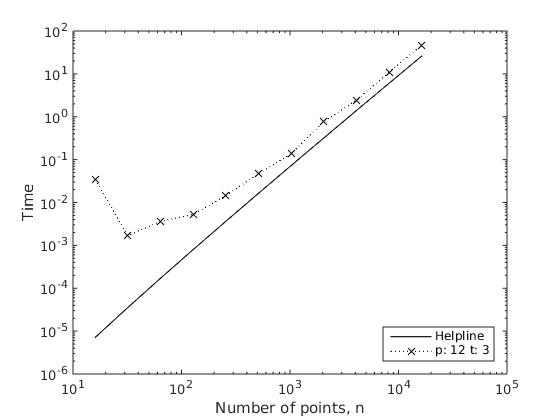
\includegraphics[width = 0.6\linewidth]{timscl}
    \caption{A loglogplot of \texttt{poisson}'s run time. The 'Helpline' shows the expected timescale, $n^2 \log_2(n)$. The dotted line is actual run time with $p = 12$, $t=3$.}
    \label{fig:timscl}
\end{figure}
The initial drop in run time is probably due to start up time and initializing. For small problem sizes the time increase is smaller than expected, but converges toward the expected timescale. The reason for the small increase in run time is due to the fact that MPI preforms better with medium problem sizes. For even lager problem sizes the run time would probably increase even faster, due to increased need to send and receive data across threads.

\subsection{Speedup analysis: MPI and OpenMP}
To compare run time, \texttt{poisson} was run with different combinations of $p$ and $t$, where $p\cdot t = 36$, and $n = 16384$. The results are shown in figure \ref{fig:time}.
\begin{figure}[h]
    \centering
    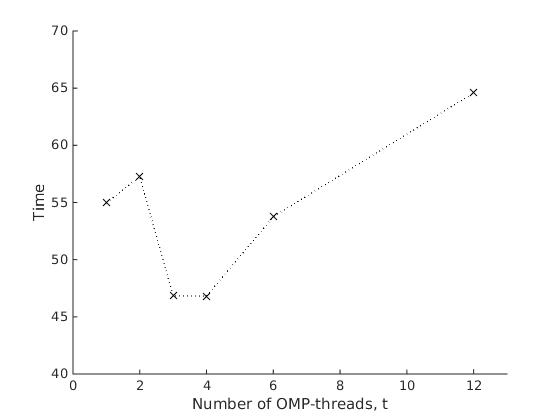
\includegraphics[width = 0.6\linewidth]{time1}
    \caption{A plot of the time used to run \texttt{poisson} with $n = 16384$ and with different numbers of MPI and OpenMP threads so that $p\cdot t = 36$. }
    \label{fig:time}
\end{figure}
From figure \ref{fig:time} we see that a combination of MPI and OpenMP threads are the optimal for solving this problem. This may be because the program was written to use both MPI and OpenMP, and without using both there are considerable extra work to do, without any gain.

\subsection{Speedup analysis: MPI} \label{sec:spup}
To measure the speedup MPI causes, \texttt{poisson} was run with $p,n$ changing and $t=1$. Figure \ref{fig:mpi} shows run time for varying $p$ when $n = 16384$. Speedup and parallel efficiency is posted in table \ref{tab:mpi}.
\begin{figure}[h]
    \centering
    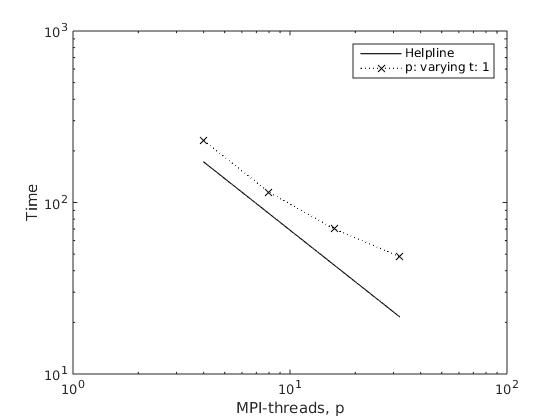
\includegraphics[width = 0.6\linewidth]{mpi}
    \caption{A plot of the time used to run \texttt{poisson} with $n = 16384$, $t = 1$, and $p$ varying.The 'Helpline' shows ideal speedup.}
    \label{fig:mpi}
\end{figure}
\begin{table}[]
\centering
\begin{tabular}{l|lllll}
$n$ & $32$ & $128$ & $1024$ & $4096$ & $16384$ \\ 
\hline
$S_4$ & 0.8137  & 1.1686  &  3.9479 & 3.9684& 3.8170 \\
$S_8$ & 0.8595 & 1.7880 & 7.4630 & 7.5402&   7.6457\\
$S_{16}$ &0.1052 & 1.5999& 11.1927 & 11.2353&  11.7548\\
$S_{32}$ &  0.0610&1.7339& 14.5749 & 17.0748& 18.6038\\
\hline
$\eta_4$ & 0.2034  &  0.2921&    0.9870&    0.9921 &   0.9543\\
$\eta_8$ &     0.1074 &   0.2235    &0.9329   & 0.9425&    0.9557\\
$\eta_{16}$&   0.0066  &  0.1000 &   0.6995  &  0.7022 &   0.7347\\
$\eta_{32}$& 0.0019  &  0.0542&    0.4555  &  0.5336 &   0.5814\\
\end{tabular}
\caption{Speedup $S_p$ and parallel efficiency $\eta_p$ for different $n,p$ with $t=1$.}
\label{tab:mpi}
\end{table}
From table \ref{tab:mpi} it is clear that using several threads on a small problem size gives little or negative gain. With larger problem sizes the speedup seems to be near perfect for few processors, and a significant increase for several processors. There also seems to be a negative speedup for $p = 4$ when $n$ goes from $4096$ to $16384$, but the numbers are to close to say anything specific, other than random interference. Figure \ref{fig:mpi} also shows the increasing speedup, and decreasing parallel efficiency.

\subsection{Speedup analysis: OpenMP}
A speedup analysis was also preformed for OpenMP. \texttt{poisson} was now run with $t,n$ changing and $p=1$. Figure \ref{fig:omp} shows run time for varying $t$ when $n = 16384$. Speedup and parallel efficiency is posted in table \ref{tab:omp}.
\begin{figure}[h]
    \centering
    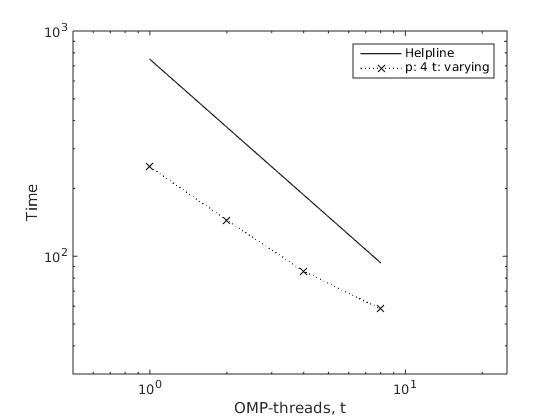
\includegraphics[width = 0.6\linewidth]{omp}
    \caption{A plot of the time used to run \texttt{poisson} with $n = 16384$, $t$ varying, and $p = 1$.The 'Helpline' shows ideal speedup.}
    \label{fig:omp}
\end{figure}
\begin{table}[h]
    \centering
    \begin{tabular}{ll|llll}
    $n$ & $32$ & $128$ & $1024$ & $4096$ & $16384$ \\ 
    \hline
    $S_4$&    2.9523&    3.5120&    3.4007&    3.8034&    3.7721\\
    $S_8$&    1.3490&    2.1090&    5.8543&    6.9255&    6.4845\\
    \hline
    $\eta_4$ &      0.7381  &  0.8780&    0.8502&    0.9508&    0.9430\\
    $\eta_8$ &      0.1686  &  0.2636&    0.7318&    0.8657&    0.8106\\
\end{tabular}
\caption{Speedup $S_t$ and parallel efficiency $\eta_t$ for different $n,t$ with $p=1$.}
\label{tab:omp}
\end{table}
From table \ref{tab:omp} it is clear that OpenMP gives a considerable speedup for both small and large problem sizes, but also seems to give a performance decrease when $n$ goes from $4096$ to $16384$. Again, this may be due to random interference, but the decrease is considerably larger than in the MPI-case. %Because of the layout of the supercomputer used; Kongull, there where not possible to get any results for $t>8$.!!!!!!!!!!!!!!!dette var dårlig skrevet, spessielt det siste!!!!!!!!!!!!!!!!!!!!!!!

\subsection{Comparing MPI and OpenMP}
When comparing speedup and parallel efficiency it is clear that MPI outperforms OpenMP for large problem sizes, and OpenMp outperforms MPI for small problem sizes. This matches the result from section \ref{sec:spup}, and it seems to be best to use a small number of OpenMP-threads, and a large number of MPI-threads. When comparing figure \ref{fig:mpi} and figure \ref{fig:omp} it may seem as OpenMP has a speedup closer to the ideal speedup, but keep in mind that the largest number of threads in figure \ref{fig:mpi} is $32$, while the largest number of threads in figure \ref{fig:omp} is $8$. Due to random interference, the results may vary, and does not give a clear answer, just indications.
%%%%%%%%%%%%%%%%%%%%%%%%%%%%%%%%%%%%%%%%%%%%%%%%%%%%%%%%%%%%%%%%%%
%%%%%%%%%%%%%%%%%%%%%%%%%%%%%%%%%%%%%%%%%%%%%%%%%%%%%%%%%%%%%%%%%%



%%%%%%%%%%%%%%%%%%%%%%%%%%%%%%%%%%%%%%%%%%%%%%%%%%%%%%%%%%%%%%%%%%
%%%%%%%%%%%%%%%%%%%%%% Changing the problem %%%%%%%%%%%%%%%%%%%%%%
%%%%%%%%%%%%%%%%%%%%%%%%%%%%%%%%%%%%%%%%%%%%%%%%%%%%%%%%%%%%%%%%%%
\section{Changing the problem}
Solving Poisson's equation on the unit square with zero boundary values is all well and good, but what happens if we want to change any of this. Let's first see what needs to change if the domain was any rectangle, that is equation (\ref{eqn:pois}) becomes
\begin{align}
  -\nabla^2 u & = f 	&\text{ in } \Omega = (0,L_x) \times (0,L_y)  \label{eqn:pois2}
\end{align}
Since we can change our reference system, any rectangular domain can be the domain in equation (\ref{eqn:pois2}). The necessary changes to \texttt{poisson} would be to create new step sizes $h_x = \frac{L_x}{n}$, and $h_y = \frac{L_y}{n}$, and change $h$ to $h_x$ and $h_y$ in the correct places. We assume that the number of interior grid points $(n-1)$ are kept equal in both directions.\\
Changing the boundary values from equation (\ref{eqn:bnd}) to
\begin{align}
 u & = g(x,y) 			&\text{ on } \partial \Omega \label{eqn:bnd2}
\end{align}
is a little more tricky. First we need to change $n-1$ internal points to $n+1$ nodes. The additional points will contain the boundary values. If $\underline{B_{old}}$ is the matrix solving (\ref{eqn:pois}) with conditions (\ref{eqn:bnd}) then $\underline{B_{new}}$ as defined in (\ref{eqn:mat}) is the matrix solving (\ref{eqn:pois}) with conditions (\ref{eqn:bnd2}).\\
\begin{align}
\underline{B_{new}} &= 
\begin{bmatrix}  
 g(x_0,y_0) & \hdots & g(x_n,y_0) \\
 \vdots &  \underline{ B_{old}} & \vdots \\
 g(x_0,y_n) & \hdots &  g(x_n,y_n)
\end{bmatrix}
\label{eqn:mat}
\end{align}
\\The two changes discussed here can easily be implemented together.

%!!!!!!!!!!!!!!!!!!!!!!Er dette rett!!!!!!!!!!!!!!!!!!!! !!!!!!!!!!!!!!!!!Det er sikkert dårlig skrevet hvertfall!!!!!!!!!!!!!!!!!!!!!!!!!!
%!!!!!!!!!!!!!!!!!!1Er dette sykt vanskelig!!!!! Eller er jeg bare nokså dum, vel duh, men likevel!!!!!!!!!!!!!!!!!

%%%%%%%%%%%%%%%%%%%%%%%%%%%%%%%%%%%%%%%%%%%%%%%%%%%%%%%%%%%%%%%%%%
%%%%%%%%%%%%%%%%%%%%%%%%%%%%%%%%%%%%%%%%%%%%%%%%%%%%%%%%%%%%%%%%%%
%We conclude from the discussion above that parallel processing is not very beneficial, and certainly not needed for our particular problem.
\section{Conclusion}
%We have revolutionised computer programming with our exceptional use of MPI and OpenMP. Both run time and convergence is clearly the best. No one has ever to create an other program solving Poisson's equation, it is done!

We have investigated the effectiveness of MPI and OpenMP on different problem sizes, with different combinations of the two. Concepts like speedup, relative efficiency and run time were measured. The convergence was good. We found that OpenMP worked well when the number of points was small, while MPI performed better when the number of points were large. When combining OpenMP with MPI we found that using a large number of MPI threads with a small number of OpenMP threads was best. \texttt{poisson} also scaled well with time vs number of points. Possible bottlenecks occur when transposing the matrix \underline{B} due to the large exchange of data between threads. 

\vspace{5cm}

\begin{thebibliography}{9}


\bibitem{kongull}
    Kongull hardware\\
    \texttt{https://www.hpc.ntnu.no/display/hpc/Kongull+Hardware}

    \bibitem{super}
    Einar M. Rønquist,
    \emph{Introduction to supercomputing},
    Problem set 4,
      2015
      
      
    \bibitem{solmeths}
    Arne Morten Kvarving,
    \emph{Introduction to supercomuting},
    Solving the linear system resulting from the Poisson problem, lecture slides,
    2015

  
  \bibitem{intro}
  Einar M. Rønquist,
  \emph{Introduction to supercomputing},
Introduction,
  2011
  \bibitem{singproc}
  Einar M. Rønquist,
  \emph{Introduction to supercomputing},
  Computer Architecture: Single Processor Systems,
  2009
  
  
  \bibitem{shell}
  Arne Morten Kvarving,
  \emph{Using the Kongull cluster},
  2012


  
\end{thebibliography}
%\bibliography{references}
\end{document}
